\documentclass[amsmath,12pt,a4paper]{amsart}
\usepackage{amsfonts, amssymb, amsmath, amscd}
\usepackage{amsthm}
\usepackage[pdftex]{graphicx}
\usepackage{multicol}
\usepackage{algorithm}
\usepackage{algpseudocode}
\usepackage{tikz}
\usepackage{ragged2e,caption}
\usepackage{pgfplots}
\pgfplotsset{compat=1.17}
\addtolength{\textheight}{4cm}
\addtolength{\voffset}{-2cm}
\addtolength{\textwidth}{5cm}%{6cm}%{4cm}
\addtolength{\hoffset}{-2cm}

\newcommand{\R}{\mathbb{R}}
\newcommand{\N}{\mathbb{N}}
\newcommand{\Z}{\mathbb{Z}}
\newcommand{\Q}{\mathbb{Q}}
\newcommand{\C}{\mathbb{C}}
\newcommand{\Bg}{\mbox{\textbf B}}
\newcommand{\vg}{\mbox{\textbf v}}
\newcommand{\ds}{\displaystyle}
\usepackage{bm,bigints, comment}
\usepackage{mathrsfs}
\usepackage{color}
\newcommand{\dpar}[2]{\dfrac{\partial #1}{\partial #2}}
\newcommand{\bu}{\mathbf{u}}
\newcommand{\bB}{\mathbf{B}}
\newcommand{\bb}{\mathbf{b}}
\newcommand{\bn}{\mathbf{n}}
\newcommand{\blam}{\mathbf{\lambda}}
\newcommand{\bbeta}{\mathbf{\beta}}
\newcommand{\balpha}{\mathbf{\alpha}}
\newtheorem{theorem}{Theorem}
\newtheorem{prop}{Proposition}
\newtheorem{Corollary}{Corollary}
\newtheorem{conj}{Conjecture}
\newtheorem{lemma}{Lemma}
\newtheorem{Remark}{Remark}
\newtheorem{Observation}{Observation}
\title[Base 64 finite compression algorithm] {Base 64 finite compression algorithm}

\author{R. Burson}

\begin{document}
\maketitle
\begin{abstract}
This work focuses on reducing base 64 data strings which is one of the most common bases used throughout computer science. We introduce the M-char inversion Theorem which which can be used on any base $64$ data set. In the corresponding algorithm we developed our own set
of symbols from drawing Trefoil knots in which we have implementing up to a $5$-char reduction technique and is out of the reach of the unicode symbols range
\end{abstract}

\section{Intro to the M-Char Reduction Map}

Let $Y$ be a string with length $m$ in base 64. Let $\mathcal{A}_m$ denote the set of strings with length $m$ of strictly capital characters $A–Z$:

$$
\mathcal{A}_m = \{ a_1a_2 \dots a_m : a_j \in \{A, B, \dots, Z\}, 1 \leq j \leq m \}.
$$

Next, let $\mathcal{S}_m$ denote all the possible string combinations of length $m$ with characters in A–Z or a–z:
\[
\mathcal{S}_m = \{ a_1a_2 \dots a_m : a_j \in \{A, B, \dots, Z\} \cup \{a, b, c, \dots, z\}, 1 \leq j \leq m \}.
\]

Now consider the set
$$
\mathcal{P}_m = \{ \xi_1, \xi_2, \dots, \xi_m : \xi_j \in \{0, 1\}, 1 \leq j \leq m \}.
$$
We call $\mathcal{P}_m$ the permutation set with modulus $m$. 

Next, take the set $\mathcal{L}_m$ to be the set of string combinations of length $m$ with at least one lowercase symbol from a–z inside of it
$$
\mathcal{L}_m = \{ \delta : \delta \in \mathcal{S}_m \setminus \mathcal{A}_m \}.
$$

Next, consider any set $\mathcal{E}_m$ of symbols with $26^m$ elements (i.e., $|\mathcal{E}_m| = 26^m$) where $m > 0$. Define the set operator $\mathcal{E}_m \, | \, \mathcal{P}_m$ as all 2-char string combinations with one element in $\mathcal{P}_m$ and the other in $\mathcal{E}_m$:
\[
\mathcal{E}_m \, | \, \mathcal{P}_m = \{ EP : E \in \mathcal{E}_m, P \in \mathcal{P}_m \}.
\]

Further, let $\mathcal{I}_m$ be the set of strings that are integers with length $m$ in base ten:
\[
\mathcal{I}_m = \{ a_1a_2 \dots a_m : a_j \in \{0, 1, 2, \dots, 9\}, 1 \leq j \leq m \}.
\]

Consider the map $\iota : \{A, B, C, \dots, Z\} \cup \{a, b, c, \dots, z\} \to \{0, 1\}$ defined as:

$$
\iota(x) = \begin{cases} 
1 & \text{if } x \in \{A, B, C, \dots, Z\}, \\
0 & \text{if } x \in \{a, b, c, \dots, z\}.
\end{cases}
$$

Finally, define $\partial : \mathcal{A}_m \to \mathcal{P}_m$ to denote the mapping that maps an M-char string to a permutation, to help identify its case sensitivity $x_1x_2x_3 \dots x_m \mapsto \left( \iota(x_1), \iota(x_2), \iota(x_3), \dots, \iota(x_m) \right)$ and $
\hbar : \mathcal{P}_m / \left\{\underbrace{(0,0,..,0)}_{m-times}\underbrace{(1,1,..,1)}_{m-times}\right\} \to \mathcal{D}_m
$to be any bijection with $|\mathcal{D}_m| = 2^m - 2$, with $\mathcal{E}_m \cap \mathcal{I}_m = \emptyset$. 

Lastly, choose any two bijections $\alpha_m : \{1, 2, \dots, 26^m\} \to \mathcal{E}_m$ and $\gamma_m : \{1, 2, \dots, 10^m\} \to \mathcal{I}_m$, and define $\mathcal{V}$ to be the set of all base 64 characters. Consider the bijection $\Xi$ from the base $\{A, B, \dots, Z\}$ to $\{a, b, c, \dots, z\}$ by taking lower cases chars and making them capital case $
\Xi(a) = A$, $\Xi(b) = B$, $\cdots$, $\Xi(z) = Z$ and also the bijection $\beta_m : \mathcal{A}_m \to \mathcal{D}_m$ defined by the rule

$$
a \mapsto \alpha_m(a)\hbar\biggl(\partial (a)\biggr) 
$$

such that

$$
\mathcal{E}_m \cap \mathcal{I}_m \cap \mathcal{D}_m \cap \mathcal{V} = \emptyset.
$$

Lastly, consider $\mho_m$ that transforms $Y$ as follows:
$$
\mho_m(Y) =
\begin{cases}
\alpha_m(Y) & \text{if } \varphi(Y) = Y \text{ and } Y \in \mathcal{A}_m \\
\beta_m(Y)  & \text{if } \varphi(Y) \neq Y \text{ and } Y \in \mathcal{L}_m \\
\gamma_m(Y) & \text{if } Y \in \mathcal{I}_m \\
Y           & \text{otherwise}
\end{cases}
$$
The map $\mho_m(Y)$ is called the $M$-char reduction map.\\

\textbf{Example 1} Let $\Sigma = \{123, AbC, AY L, lli, +ill, Y AC, bA3, 32t, U\}$ and consider all subsets that have the same order in chunks of at most three elements:
$$
\{123\}, \{AbC\}, \{AY L\}, \{lli\}, \{+ill\}, \{Y AC\}, \{bA3\}, \{32t\}, \{U\}.
$$

Take any $3$-char string $Y$ from these particular subsets (i.e., $Y := AbC$). Let $\mathcal{C}$ be the set of all Chinese symbols in the Unicode range $[0x4E00, 0x9FFF]$. Let $\mathcal{J}$ denote the set of Japanese symbols from the ranges $[0x3040, 0x309F]$, $[0x30A0, 0x30FF]$, and $[0x4E00, 0x9FFF]$, and $[0x31F0, 0x31FF]$. Define $\mathcal{D}$ as the set of $48$ Cambodian symbols in the range $[0x1780, 0x17FF]$. Let $\mathcal{C}^\prime$ be a subset of $\mathcal{C}$ such that $|\mathcal{C}^\prime| = (2^3-2)$, $\mathcal{J}^\prime$ be a subset of $\mathcal{J}$ such that $|\mathcal{J}^\prime| = 103$, and $\mathcal{D}^\prime$ be any subset of $\mathcal{D}$ with $|\mathcal{D}^\prime| = (2^3 - 2)$. Consider two bijections $\alpha : \{1, 2, 3, \ldots, 26^3\} \to \mathcal{C}^\prime$, $\gamma : \{1, 2, 3, \ldots, 10^3\} \to \mathcal{J}$, and $\beta$ explicitly defined as

$$
a \mapsto \alpha(a)\hbar \biggl(\partial (a)\biggr)
$$

Lastly, consider the reduction map $\mho_3(Y)$:

$$
Y \mapsto 
\begin{cases}
\alpha(Y) & \text{if } \varphi(Y) = Y \text{ and } Y \in \mathcal{A}_3, \\
\beta(Y)  & \text{if } \varphi(Y) \neq Y \text{ and } Y \in \mathcal{L}_3, \\
\gamma(Y) & \text{if } Y \in \mathcal{I}_3, \\
Y         & \text{otherwise}.
\end{cases}
$$

Then we represent the entire string using the image:
$$
\mho_3(\Sigma) = \gamma(123) \beta(AbC) \alpha(AYL) \beta(lli) + ill \alpha(Y AC) bA332tU,
$$
which is 19 characters compared to 26 originally.\\


\textbf{Example 2}: Take $\Sigma = \{123AbCJKII + INJ\}$ and set $m = 3$. Let $\mathcal{C}$ denote the set of all Chinese symbols specifically in the Unicode range $[0x4E00, 0x88D7]$ with cardinality $|\mathcal{C}| = 26^3$, and let $
\mathcal{D} = \{\spadesuit, \diamondsuit, \emptyset, \Game,\blacktriangle , \blacktriangledown\}.
$. Take $\hbar: \mathcal{P}_3 / \{(0, 0, 0), (1, 1, 1)\} \to \mathcal{D}$ to be the bijection

 \begin{equation*}
\begin{split}
\hbar(0,0,1) & = \Game\\
\hbar(0,1,1) & = \lozenge\\
\hbar(0,1,0) & = \emptyset\\
\hbar(1,1,0) & = \blacktriangle\\
\hbar(1,0,0) & = \blacktriangledown\\
\hbar(1,0,1) & = \spadesuit
\end{split}
\end{equation*} Set $\mathcal{E}$ to denote the set of all emoji symbols available in Unicode (there are more than 3,600). Take any subset $K \subset \mathcal{E}$ such that $|K| = 1000$ and take two bijections $\gamma : \mathcal{I}_3 \to K$ and $\alpha : \mathcal{A}_3 \to \mathcal{C}$. Then take the bijection $\beta : \mathcal{A}_3 \to \mathcal{C} \cup \mathcal{D}$ using the rule:
$$
a \mapsto \alpha(a) \hbar \left( \partial(a) \right).
$$

We set the reduction map $\mho_3(Y)$:
\begin{equation}
Y \mapsto 
\begin{cases}
\alpha(Y) & \text{if } \varphi(Y) = Y \text{ and } Y \in \mathcal{A}_3, \\
\beta(Y)  & \text{if } \varphi(Y) \neq Y \text{ and } Y \in \mathcal{L}_3, \\
\gamma(Y) & \text{if } Y \in \mathcal{I}_3, \\
Y         & \text{otherwise}.
\end{cases}
\end{equation}

Then, representing $\Sigma$ as an ordered string, we have:
$$
\Sigma  = \gamma(123) \beta(AbC) \alpha(JNK) II + \alpha(INJ) =  \gamma(123) \gamma(ABC)\spadesuit \alpha(JNK) II + \alpha(INJ)$$


\textbf{Example 3}:
This example skips the bijection definitions since the reader can clarify if the context is provided. Using $\Sigma = \{AxBIJKY + YY12356RD\}$, we can separate it into seven organized sets

$$
\{AxB\}, \{IJK\}, \{Y + Y\}, \{Y\}, \{123\}, \{56R\}, \{D\}.
$$

Then, we have

\begin{align*}
AxB & \mapsto \beta \Delta \quad \text{(1-char Chinese string with 1-char Khmer attachment)} \\
IJK & \mapsto \alpha \quad \text{(1-char Chinese string)} \\
Y + Y & \mapsto Y + Y \quad \text{(identity map)} \\
Y & \mapsto Y \quad \text{(identity map)} \\
123 & \mapsto \Upsilon \quad \text{(1-char Japanese string)} \\
56R & \mapsto 56R \quad \text{(identity map)} \\
D & \mapsto D \quad \text{(identity map)} \\
\end{align*}

Hence, the result is
$$
\Sigma = "AxBIJKY + YY12356RD" = "B\Delta \alpha Y + YY \Upsilon 56RD",\indent \textbf{17 chars vs. 12}
$$

\section{M-char index assigning and inverse reduction using Euclidean algorithm}
In this section we start by introducing the M-char inverse theorem using an example.\\

Set $m = 4$ and take the set $\mathcal{A}_4$ (as introduced in the introduction in section 1). Take the ordered base of all capital letters in the English alphabet $B = \{A, B, C, \ldots, Z\}$. Since $B$ is finite and no elements repeat, there is a bijection $Z : \{1, 2, \ldots, |B|\} \to B$ so that $Z^{-1}(b) = i$ with $i$ being unique for each $b \in B$. Take the mapping $\wp_4 : \mathcal{A}_4 \to \mathbb{N}^4$ that takes in a 4-char word, say $b = b_1b_2b_3b_4$, and maps it to a vector in $\mathbb{N}^4$ (with each component being less than the cardinality of the base) using the rule:

$$
b = b_1b_2b_3b_4 \mapsto (Z^{-1}(b_1), Z^{-1}(b_2), Z^{-1}(b_3), Z^{-1}(b_4)).
$$

Here $Z^{-1}$ denotes the inverse of the bijection $Z$, so that it maps each character to an index in the base, in this case, $1 - 26$. Next, consider that the map $\wp_4$ maps the $4$-char word to an index in $\{1, 2, \ldots, |B|^m\}$ using the base formula

$$
b = b_1b_2\ldots b_4 \mapsto \left( \sum_{n=1}^{3} 26^{4-n} \left( Z^{-1}(b_n) - 1 \right) \right) + Z^{-1}(b_4).
$$

For visual purposes, we display the map:
$$\begin{aligned}
&AAAA \mapsto 26^3(0) + 26^2(0) + 26^1(0) + 1 = 1, \\
&AAAB \mapsto 26^3(0) + 26^2(0) + 26^1(0) + 2 = 2, \\
&\vdots \\
&AABA \mapsto 26^3(0) + 26^2(0) + 26^1(1) + 1 = 27, \\
&\vdots \\
&ZZZZ \mapsto 26^3(25) + 26^2(25) + 26^1(25) + 26 = 264.
\end{aligned}$$

Now consider the intermediate mapping $\wp^{-}_4$ (the intermediate inverse):
$$
\wp^{-}_4(x) =
\begin{cases}
(1, 1, 1, x), & \text{if } 1 \leq x \leq |\mathcal{B}| \\
(1, 1, q + 1, r), & \text{if } |\mathcal{B}| < x < |\mathcal{B}|^2, \, x = q|\mathcal{B}| + r \\
(1, 1, |\mathcal{B}|, |\mathcal{B}|), & \text{if } x = |\mathcal{B}|^2 \\
(1, q + 1, k + 1, l), & \text{if } |\mathcal{B}|^2 < x < |\mathcal{B}|^3, \, x = q|\mathcal{B}|^2 + r, \, r = k|\mathcal{B}| + l \\
(1, |\mathcal{B}|, |\mathcal{B}|, |\mathcal{B}|), & \text{if } x = |\mathcal{B}|^3 \\
(h + 1, q + 1, f + 1, l), & \text{if } |\mathcal{B}|^3 < x < |\mathcal{B}|^4, \, x = h|\mathcal{B}|^3 + r, \, r = q|\mathcal{B}|^2 + k, \\
k = f|\mathcal{B}| + l \\
(|\mathcal{B}|, |\mathcal{B}|, |\mathcal{B}|, |\mathcal{B}|), & \text{if } x = |\mathcal{B}|^4
\end{cases}
$$

Then take $\Gamma : \{1, 2, \ldots, |\mathcal{B}|^4\} \to \mathcal{A}_4$ defined as

$$
\Gamma(x) = \sum_{j=1}^{4}{ Z(\wp^{-}_4(x)_j)}
$$

where $Z$ takes in an index and maps to a letter $\{A, B, C, \cdots, Z\}$. The operator $\Sigma$ takes in an element from $\{A, B, C, \cdots, Z\}$ and concatenates it with another string (adding string $A + A = AA$). Similarly, $\wp^{-}_j$ denotes the $j^th$ coordinate of the vector $\wp^{-}$. As an example, take $x = 27 = 26 \cdot 1 + 1$, as a result we have

$$
x \mapsto (1, 1, q + 1, r) = (1, 1, 1 + 1, 1) = (1, 1, 2, 1) \mapsto AABA.
$$

Similarly,

$$
677 = 26^2 \cdot 1 + 1 \mapsto (1, 2, 1, 1) \mapsto ABAA.
$$

\textbf{Lemma 1.} Let $m \in \mathbb{N}$ with $m > 1$ and let $Z : \{1, 2, \ldots, |\mathcal{B}|\} \to \mathcal{B}$ denote any bijection with inverse $Z^{-}$. The map $\Gamma : \mathcal{A}_m \to \{1, 2, 3, \ldots, |\mathcal{B}|^m\}$ defined by the rule

$$
b = b_1b_2 \ldots b_m \mapsto \left( \sum_{n=0}^{m-1} |B|^{m-n} \left( Z^{-}(b_n) - 1 \right) \right) + Z^{-}(b_m)
$$
is a bijection.\\

\textbf{Proof.} First let $a, b \in A_m$. Assume $\Gamma(a) = \Gamma(b)$, then immediately 


\begin{equation}
\begin{split}
\sum_{n=0}^{m-1} |\mathcal{B}|^{m-n} \left( Z^{-}(a_n) - 1 \right) &= \sum_{n=0}^{m-1} |\mathcal{B}|^{m-n} \left( Z^{-}(b_n) - 1 \right) \\
&\Downarrow \\
\sum_{n=0}^{m-1} |\mathcal{B}|^{m-n} \left( (Z^{-}(a_n) - 1) + (Z^{-}(b_n) - 1) \right) &= 0 \\
&\Downarrow \\
(Z^{-}(a_n) - 1) + m (Z^{-}(b_n) - 1) &= 0 \\
&\Downarrow \\
a_n &= b_n \quad \forall n \in \{1, 2, 3, \ldots, m\} \\
\\
a &= b
\end{split}
\end{equation}


Next, choose arbitrarily $b \in \{1, 2, 3, \ldots, |\mathcal{B}|^m\}$. We must show that there exists an $a$ such that $\Gamma(a) = b$. We break it up using cases and the Euclidean algorithm. For arbitrary $b > |\mathcal{B}|$, consider the sequence $\{q_1, q_2, \ldots, q_{m-1}\}$ determined by solving the following set of equations using the Euclidean algorithm:

$$
\begin{cases}
b &= q_1|\mathcal{B}| + r_1 \indent \text{if $|\mathcal{B}| < b \leq |\mathcal{B}|^2$} \\
b& = q_1|\mathcal{B}|^2 + r_1, \, r_1 = q_3|\mathcal{B}| + r_3, \indent \text{if $|\mathcal{B}|^2 < b \leq |\mathcal{B}|^3$} \\
\vdots \\
b &= q_1|\mathcal{B}|^{m-1} + r_1, \, r_1 = q_3|\mathcal{B}|^{m-2} + r_3, \, r_3 = q_4|\mathcal{B}|^{m-3} + r_5, \ldots, \, r_{m-1} = q_m|\mathcal{B}| + r_m
\end{cases}
$$

and $s = r_k$ for some $k$ determined by finding the vector $(k, k + 1)$ so that $|\mathcal{B}|^k \leq b \leq |\mathcal{B}|^{k+1}$. Next, consider the intermediate mapping $\wp : \mathbb{N} \to \mathbb{N}^4$:

\begin{equation}
b \mapsto
\begin{cases}
(\underbrace{1, \ldots, 1, 1, 1,\cdots}_{m-1~ times} , b), &\indent \text{if  $1 \leq b \leq |\mathcal{B}| $}\\
(\underbrace{1,1, 1,\cdots}_{m-2 ~times}, q_1 + 1, s), & \indent\text{if $ |\mathcal{B}| < b < |\mathcal{B}|^2$} \\
(1, 1, 1, \ldots, \underbrace{|\mathcal{B}|, |\mathcal{B}|)}_{2-times} & \text{if } b = |\mathcal{B}|^2 \\
\vdots \\
(q_1 + 1, q_2 + 1, q_3 + 1, \ldots, q_{m-1} + 1, s) & \text{if } |\mathcal{B}|^{m-1} < b < |\mathcal{B}|^m \\
(\underbrace{|\mathcal{B}|, |\mathcal{B}|, |\mathcal{B}|, \ldots, |\mathcal{B}|}_{m-times} ) & \indent \text{if $b = |\mathcal{B}|^m$}
\end{cases}
\end{equation}

$$
a = \sum_{j=1}^m Z(\wp(a)_j)
$$

then $\Gamma(a) = b$ (recall that if the parameter of \(\Sigma\) is a string, it adds them similarly to addition).

\begin{theorem}(Gene realized $M$-char inversion theorem)
Set \(m \in \mathbb{N}\), \(\mathcal{B} = \{A, B, C, \ldots, Z\}\), and let \(Z : \{1, 2, \ldots, |\mathcal{B}|\} \to \mathcal{B}\) denote any bijection with inverse \(Z^{-}\). Define the map \(\wp_m : \mathbb{N} \to \mathbb{N}^m\) as follows:

\begin{equation}
n \mapsto
\begin{cases}
(1, \ldots, 1, 1, 1 \quad 1, n), & ~~ \text{if $1 \leq n \leq |\mathcal{B}|$} \\
(1, \ldots, 1, 1, 1 1, q_1 + 1, s), & ~~\text{if $|\mathcal{B}| < n < |\mathcal{B}|^2$} \\
(1, 1, 1, \ldots, |\mathcal{B}|, |\mathcal{B}|) &~~ \text{if $n = |\mathcal{B}|^2$} \\
\vdots \\
(q_1 + 1, q_2 + 1, q_3 + 1, \ldots, q_{m-1} + 1, s) &~~\text{if $|\mathcal{B}|^{m-1} < n < |\mathcal{B}|^m$} \\
(|\mathcal{B}|, |\mathcal{B}|, |\mathcal{B}|, \ldots, |\mathcal{B}| \quad |) & \indent \text{if $n = |\mathcal{B}|^m$}
\end{cases}
\end{equation}

with \(q_j : \{1, 2, \ldots, m - 1\} \to \{0, 1, 2, \ldots, (|\mathcal{B}| - 1)\}\) being the sequence \(\{q_1, q_2, \ldots, q_{m-1}\}\) determined by solving the following set of equations using the Euclidean algorithm:

$$
\begin{cases}
n = q_1|\mathcal{B}| + r_1 & \text{if $|\mathcal{B}| < n \leq |\mathcal{B}|^2$} \\
n = q_1|\mathcal{B}|^2 + r_1, \, r_1 = q_3|\mathcal{B}| + r_3 & \text{if $|\mathcal{B}|^2 < n \leq |\mathcal{B}|^3$} \\
\vdots \\
n = q_1|\mathcal{B}|^{m-1} + r_1, \, r_1 = q_3|\mathcal{B}|^{m-2} + r_3, \, r_3 = & q_4|\mathcal{B}|^{m-3} + r_5,  \ldots, \, r_{m-1} = q_m|\mathcal{B}| + r_m 
\end{cases}
$$

and $s = r_k$ for some $k$ determined by finding the vector $(k, k + 1)$ so that $|\mathcal{B}|^k \leq n \leq |\mathcal{B}|^{k+1}$.

Then the mapping $\Gamma : \{1, 2, \ldots, |\mathcal{B}|^m\} \to A^m$ is defined by

$$
n \mapsto \sum_{j=1}^m Z(\wp(n)_j)
$$

which is the inverse of $\Gamma^{-} : A^m \to \{1, 2, \ldots, |\mathcal{B}|^m\}$ given by

$$
b = b_1 b_2 \ldots b_m \mapsto \sum_{n=1}^{m-1} |\mathcal{B}|^{m-n} \left( Z^{-}(b_n) - 1 \right) + Z^{-}(b_m)
$$
\end{theorem}


\section{Creating $\mathcal{B}^m-1$ transformations}
In this section, we introduce an efficient method to generate enough string characters in order to establish the necessary bijection for the decryption process. Technically, regardless of whether or not one has established a bijection, the data gathered from reducing the base 64 string will be the same even if the M-char reduction mapping is not surjective; we just need to make sure every M-char is mapped to some element that is a 1-char. We consider a set of points in the cross-section of a Trefoil knot \(T : [0, 2\pi] \to \mathbb{R}^2\):

\begin{center}
% Trefoil knot with closer tick marks and a second smaller dampened knot

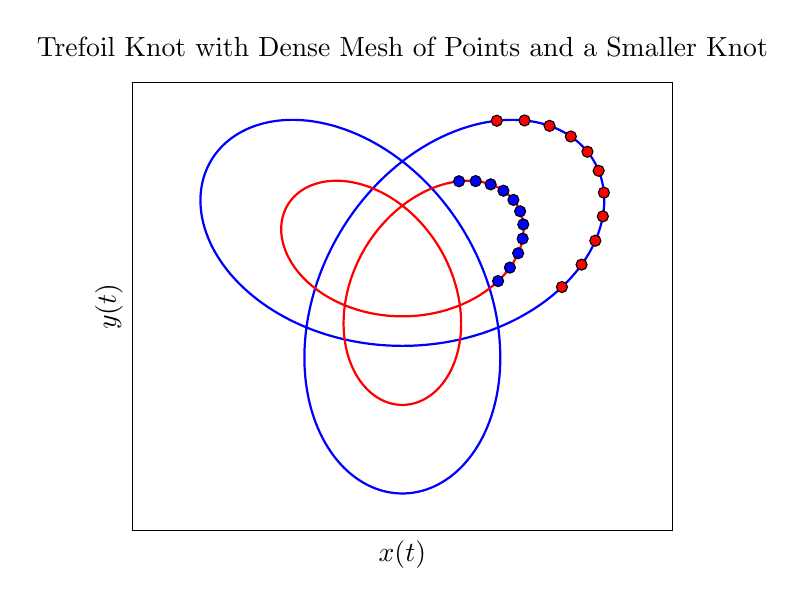
\begin{tikzpicture}
    \begin{axis}[
        axis equal,
        ticks=none,
        xlabel={$x(t)$},
        ylabel={$y(t)$},
        title={Trefoil Knot with Dense Mesh of Points and a Smaller Knot},
        enlargelimits=true
    ]

    % Original knot (blue curve) with red mesh points
    \addplot[
        domain=0:6.2832, % 0 to 2pi
        samples=2000,
        thick,
        smooth,
        color=blue
    ] 
    ({sin(deg(x)) + 2*sin(deg(2*x))}, {cos(deg(x)) - 2*cos(deg(2*x))});
    
    % Red mesh points for original knot
    \addplot[
        only marks,
        mark=*,
        mark options={fill=red, draw=black},
        samples at={0.5, 0.6, 0.7, 0.8, 0.9, 1.0, 1.1, 1.2, 1.3, 1.4, 1.5}
    ] 
    ({sin(deg(x)) + 2*sin(deg(2*x))}, {cos(deg(x)) - 2*cos(deg(2*x))});
    
    % Add labels for the mesh points (very close together)
    \node at (axis cs: 1.15, 1.4) [anchor=south west, font=\tiny] {};
    \node at (axis cs: 0.95, 1.25) [anchor=south west, font=\tiny] {};
    \node at (axis cs: 0.75, 1.1) [anchor=south west, font=\tiny] {};
    \node at (axis cs: 0.55, 0.95) [anchor=south west, font=\tiny] {};
    \node at (axis cs: 0.35, 0.8) [anchor=south west, font=\tiny] {};
    \node at (axis cs: 0.15, 0.65) [anchor=south west, font=\tiny] {};
    \node at (axis cs: -0.05, 0.5) [anchor=south west, font=\tiny] {};
    \node at (axis cs: -0.25, 0.35) [anchor=south west, font=\tiny] {};
    \node at (axis cs: -0.45, 0.2) [anchor=south west, font=\tiny] {};
    \node at (axis cs: -0.65, 0.05) [anchor=south west, font=\tiny] {};
    \node at (axis cs: -0.85, -0.1) [anchor=south west, font=\tiny] {};

    % Smaller, dampened knot (red curve)
    \addplot[
        domain=0:6.2832,
        samples=2000,
        thick,
        smooth,
        color=red
    ]
    ({0.6*(sin(deg(x)) + 2*sin(deg(2*x)))}, {0.6*(cos(deg(x)) - 2*cos(deg(2*x)))});
    
    % Blue mesh points for smaller dampened knot
    \addplot[
        only marks,
        mark=*,
        mark options={fill=blue, draw=black},
        samples at={0.5, 0.6, 0.7, 0.8, 0.9, 1.0, 1.1, 1.2, 1.3, 1.4, 1.5}
    ]
    ({0.6*(sin(deg(x)) + 2*sin(deg(2*x)))}, {0.6*(cos(deg(x)) - 2*cos(deg(2*x)))});
    
    \end{axis}
\end{tikzpicture}

\end{center}

$$
\mathcal{T}_1 = \{ (x(t), y(t)) : t \in [0, 2\pi] \}
$$

where

\[
x(t) = \sin(t) + 2 \sin(2t),
\]
\[
y(t) = \cos(t) - 2 \cos(2t).
\]

We define the set of \(|\mathcal{B}|^m - 1\) transformations using a coordinate transformation mapping:

$$
\mathcal{T}_k = \{ v : v = \frac{1}{p(k)} T, T \in T_1, P(k) = \frac{1}{k} \}
$$
for $k \leq |\mathcal{B}|^m - 1$. We start with a mesh size of $2000$ values:

$$
t \in \left\{ \frac{k(2\pi)}{2000} : k \in \{0, 1, 2, \ldots, 1999\} \right\} := T.
$$

Each set of points in \(\{(x(t), y(t)) : (x(t), y(t)) \in T_1 \text{ and } t \in T\} \subset T_1\) is compacted to a canvas, and we draw a symbol using a straight-line method from point to point \((x(t_i), y(t_i))\) to \((x(t_{i+1}), y(t_{i+1}))\). Then, we further save each symbol as a 1-char string, similar to how Unicode is created. This method avoids calculating a new set of points (or symbols) each time; instead, we use a transformation of one symbol in our case, a Trefoil knot.

\section{Results and Data}

In this section, we attach and report the results we found for our implementation of the base 64 finite compression algorithm using a 3-char, 4-char, and 5-char reduction technique.

\begin{table}[h]
    \centering
    \caption{Results using 3-char reduction on sample data.}
    \begin{tabular}{|c|c|c|c|}
        \hline
        Test & Base 64 Length & Encrypted Length & Decrease Amount \\
        \hline
        1 & 3085 & 1540 & 2.003 \\
        2 & 3335 & 1594 & 2.105 \\
        3 & 4650 & 2351 & 1.978 \\
        4 & 5493 & 2703 & 2.032 \\
        5 & 5814 & 2918 & 1.992 \\
        6 & 6650 & 3281 & 2.027 \\
        \hline
    \end{tabular}
\end{table}

\begin{table}[h]
    \centering
    \caption{Results using 4-char reduction on sample data.}
    \begin{tabular}{|c|c|c|c|}
        \hline
        Test & Base 64 Length & Encrypted Length & Decrease Amount \\
        \hline
        1 & 864 & 237 & 3.64 \\
        2 & 1499 & 466 & 3.217 \\
        3 & 1149 & 459 & 2.503 \\
        4 & 1169 & 183 & 6.388 \\
        5 & 1863 & 481 & 3.873 \\
        6 & 2556 & 836 & 3.057 \\
        \hline
    \end{tabular}
\end{table}


\section{Compression Tool Overview}

The Compression tool is publicly available inside of the server file on GitHub and is currently being enhanced. It will be compacted into a separate file when completed. The decompression tool is experiencing issues; while the symbols are being drawn, we have detected that they are not being made uniquely. To compensate for this, we have commented out this portion of the code and are now currently using Unicode testing when the modulus \( m = 3 \). This section will be updated when this code is complete. The compression tool is functioning when we use a unique subset of Unicode symbols, but it does not work properly when we attempt to create our own symbols. We have failed to do this correctly. We state that we have successfully conducted a $5$-char reduction technique because it does not matter if the strings that we created and mapped to are unique or not since the data will not change in this case. We have successfully created $26^5$ symbols, but we have detected that they are not unique. Thus, we are converting to a transformation of Trefoil knots; in previous applications, we were using spirals with increasing angles. The symbols only need to be unique for the decompression tool to work properly; this does not significantly affect the results that one can gather. We are currently working on fixing this issue by testing with Unicode symbols. The algorithm is robust, allowing the user to call it with their own symbols inside an array. The compression function is titled \texttt{BursonBase64Encrypted()} and the decompression tool is titled \texttt{BursonBase64Decrypt()}. For any application, we recommend using the function \texttt{getModCharInverse()} to increase the speed of creating the inverse map for the three sets of data that one needs, as it can be used on all three sets and also called in the same loop while initializing their own symbols.One does not need to add an additional loop to create the inverse set; our code will automatically create it if one calls it properly and pushes the inverse symbol data created directly under where they append to the array storing their own unique symbols. The function \texttt{getModCharInverse()} takes in the index of your inverse array, the modulus, and the base set. For example, set your base to \( \mathcal{B} = \{ A, B, C, \ldots, Z \} = \texttt{"ABC...Z"} \) as an ordered string, and our function produces results

\begin{align*}
\texttt{getModCharInverse(1, 4, B)} &= \texttt{"AAAA"} \\
\texttt{getModCharInverse(2, 4, B)} &= \texttt{"AAAB"} \\
\texttt{getModCharInverse(1, 5, B)} &= \texttt{"AAAAA"} \\
\texttt{getModCharInverse(265 - 1, 5, B)} &= \texttt{"ZZZZY"}
\end{align*}

We are currently calling it inside the same loop where we assign the Unicode to the array, and it is giving consistent inverse results for both our main set and our permutation set (but it returns a string representation, i.e., \( 101010 \) for our permutation \( (1, 0, 1, 0, 0) \), which can easily be applied to our reduced symbol in \( A^4 \)). 

It is rather sophisticated and can easily be adapted inside any code to create inverses of many arrays, regardless of the data type.

\section{Future work}

Any future work that attempts to enhance the algorithm introduced in this work needs to increase the modulus from a 5-char reduction to a 6-char or 7-char reduction and possibly above, as we have already been able to gather data from this range of modulus. We are unsure exactly how many unique string characters we can physically create and compact to a 1-char string; this needs further investigation. Moreover, the method we use to organize the sets that we perform the reduction on is allowed to be arbitrary, as long as we preserve the order and only perform a reduction mapping on elements that are the same modulus as \( m \). In fact, many times under the application of the algorithm, there exist sets that cannot be organized easily with \( m - 1 \) or \( m - \epsilon \) elements inside. For each \( m \), one can also reduce each set that has less cardinality than \( m \) itself. The number of elements we need to perform the reduction technique is given by the formula

\[
f(m) = 26^m + 10^m + (2^m - 2) + 4
\]

Namely, \( 26^m \) elements to reduce a string \( a \in A^m \) since each character can correspond to one of the elements in \( \{1, 2, \ldots, |B| = 26\} \). Instead of mapping the chunks with \( m - \epsilon \) length (with \( 1 \leq \epsilon \leq m - 1 \)) to the identity map in \( f_m \), if one wants to reduce all the organized subsets that have been organized, then the algorithm needs to efficiently create \( \lambda(m) \) elements with

\[
\lambda(m) := \sum_{i=1}^{m} f(i) - 4 + 4 = \left( \sum_{i=1}^{m} 26^i + 10^i + 2^i \right) - 2m + 4.
\]

One can easily see this because for each set of unique symbols, say \( O_i \), that one needs to create, the cardinality must satisfy \( |O_i| \geq f(i) - 4 \) and \( |O_i \cap O_j| = \emptyset \) for any \( i \neq j \) and \( 1 \leq j \leq f(m) - 4 \). 

One needs \( 10m \) elements to reduce string chunks of length \( m \) that are strictly integers since these characters are in base 10, and then one needs \( 2m - 2 \) unique permutations in \( P_m \) to permute each element in \( A^m \) besides all capital or lower case possibilities. Lastly, we need the four symbols set \( \sim, |, \$, \) and \( 0 \): the prime symbol indicating lower case combinations, with \( \sim \) separating an encrypted number from a reduced pattern (i.e., \( 10|\gamma = \gamma\gamma\gamma\gamma\gamma\gamma\gamma\gamma\gamma\gamma \) versus \( 10 \gamma = 10\gamma \)) and also the dollar symbol \( \$ \) and \( [ \) to perform the Owlpha loop technique located inside the algorithm. It is ideal for the algorithm to build \( \lambda(m) \) unique Trefoil knots, which one can store in multiple arrays (as the maximum array size will fill up rather quickly), and then the case statements need to be altered in a fashion so that one does not have to manually set the data from the modulus, but rather only change the modulus and gather results.

\section{Conclusion}
This algorithm was initially built intending to reduce a set of one thousand base 64 images that will be saved to a $ERC1155$ block chain contract representing NFT tokens. Our intention is not to change or alter our allotted $512MB$ limitation but rather use the $M$-char reduction technique introduced in this work to compress the data and after convert it by saving the existing data onto our contract rather then to our existing database to save production cost. We have successful outlined and performed the base 64 reduction technique introduced in this work on sample and real existing string data using a $M$-char reduction technique for $M \le 5$ as well as provided the
necessary mathematical framework necessary to formally introduce our technique. The technique outlined in this work can be used on any data set to reduce the current amount of storage inside a
database or on a block chain contract (which can hold the data instead which reduced production cost long term). Moreover, we have also outlined and discussed methods to enhance the algorithm.
Ultimately, this works effectively shows their is a need to study and enhance the algorithm we provided to increase the amount of data that one can store rather then enhancing than technology
that stores the data. There are many practical application of the M-char reduction technique including (but are not limited to) sending more data through satellites, storing more data in a
database or block chain contract, possibly speeding up calculating and more.

\bibliographystyle{amsplain}
\end{document}
